\chapter{Lokale Quantenfelder und die eindimensionale Dirac-Gleichung}

Quantenfelder haben wir bereits anhand ihrer Quanten, ihrer Erzeugungs- und Vernichtungsoperatoren und des einfachsten Hamiltonoperators für nichtrelativistische Teilchen kennengelernt. Nun wollen wir mit diesem Apparat etwas anfangen. Zunächst werden wir nicht nur behaupten, sondern auch zeigen, wie ein räumlich lokaler Hamiltonoperator den Impuls erhält. Dann lassen wir Produkte von Feldern Streuung und Zerfall beschreiben und verfolgen, wie wiederholtes Wirken des Hamiltonoperators die Anfänge der diagrammatischen Störungstheorie hervorbringt. Erst danach wenden wir uns dem angekündigten Fermionenproblem zu. Der einfachste Einstieg führt noch nicht über ein Fermionenfeld, sondern über die eindimensionale Dirac-Gleichung.

\section{Noch einmal der Feld-Hamiltonoperator}

Der Hamiltonoperator für eine Sorte nichtrelativistischer Teilchen lautet
\begin{equation}
H_0=\int dx\,
\psi^\dagger(x)
\left[-\frac{\partial_x^2}{2m}+V(x)\right]
\psi(x).
\label{eq:l9-nonrel-hamiltonian}
\end{equation}
Die Schreibweise wirkt eindimensional, doch nichts im einleitenden Argument hängt von dieser Einschränkung ab: In drei Dimensionen kann \(x\) für den Vektor \(\mathbf{x}\) stehen, \(dx\) für \(d^3x\) und \(-\partial_x^2\) für \(-\nabla^2\).

Der Operator \(\psi^\dagger(x)\) erzeugt bei \(x\) ein Teilchen, während \(\psi(x)\) dort eines vernichtet. Ihr normalgeordnetes Produkt
\begin{equation}
n(x)=\psi^\dagger(x)\psi(x)
\end{equation}
ist die lokale Teilchenzahldichte. Der Potentialterm lautet daher
\begin{equation}
H_V=\int dx\,V(x)n(x).
\end{equation}
Genau so würden wir es für ein klassisches Gas schreiben: Wir zählen die Teilchen in der Nähe von \(x\), weisen jedem die potentielle Energie \(V(x)\) zu und summieren über den Raum. Zu diesem Zeitpunkt wechselwirken die Teilchen nicht miteinander. Sie können auf ein von außen angelegtes Potential reagieren, aber im Übrigen ist der Hamiltonoperator eine Summe unabhängiger Einteilchenenergien.

Es ist hilfreich, den Ausdruck zunächst zu vereinfachen und dann zum Ausgangspunkt zurückzukehren. Setzen wir das Potential gleich einer Konstanten, \(V(x)=V_0\). Ein konstantes Potential übt keine Kraft aus, doch seine Bedeutung als Operator ist unmittelbar einsichtig:
\begin{equation}
\begin{aligned}
H_V&=V_0\int dx\,\psi^\dagger(x)\psi(x)=V_0N,\\
N&=\int dx\,n(x).
\end{aligned}
\end{equation}
Es verleiht jedem Teilchen dieselbe additive Energie. Um die Ruheenergie in einer nichtrelativistischen Beschreibung beizubehalten, wählen wir \(V_0=mc^2\). Der Term zählt dann für jedes Teilchen eine Ruheenergie. Diese ansonsten belanglose Konstante behalten wir bei, weil sie die Translationsinvarianz erhält und den Zählvorgang sichtbar macht.

\section{Der Hamiltonoperator als Aktualisierungsvorschrift}

Was bedeutet die Aussage, dass der Impuls erhalten ist? Die Antwort sollten wir damit formulieren, was der Hamiltonoperator bewirkt. Um \(\psi\) nicht gleichzeitig für einen Feldoperator, eine Einteilchenwellenfunktion und einen Vielteilchenzustand zu verwenden, bezeichnen wir den Vielteilchenzustand mit \(\lvert\Phi(t)\rangle\). Während eines kurzen Zeitintervalls \(\epsilon\) gilt
\begin{equation}
\lvert\Phi(t+\epsilon)\rangle
=\left(1-i\epsilon H+O(\epsilon^2)\right)
\lvert\Phi(t)\rangle,
\label{eq:l9-short-update}
\end{equation}
wobei \(\hbar=1\). Der erste Term ist der unveränderte Zustand; die erste Korrektur wird durch \(H\) erzeugt. Wiederholtes Anwenden dieser Aktualisierung führt zur Schr\"odinger-Gleichung.

Die Impulserhaltung hat nun eine konkrete Bedeutung. Hat der Anfangszustand einen bestimmten Gesamtimpuls \(P\), so muss \(H\lvert\Phi\rangle\) denselben Gesamtimpuls haben. Andere Eigenschaften können sich ändern und einzelne Teilchen können Impuls austauschen, aber der Hamiltonoperator darf den Zustand nicht in einen Sektor mit anderem Gesamt\(P\) überführen. Wir können dies direkt überprüfen, indem wir den Hamiltonoperator in der Impulsbasis umschreiben.

\section{Das räumliche Integral als Impuls-Deltafunktion}

Wir wählen die Fourier-Konvention
\begin{align}
\psi(x)&=\int\frac{dp}{\sqrt{2\pi}}\,a(p)e^{ipx},\\
\psi^\dagger(x)&=\int\frac{dq}{\sqrt{2\pi}}\,a^\dagger(q)e^{-iqx}.
\label{eq:l9-field-fourier}
\end{align}
Der Operator \(a(p)\) vernichtet ein Teilchen mit Impuls \(p\). Der Operator \(a^\dagger(q)\) erzeugt ein Teilchen mit Impuls \(q\). Die verschiedenen Buchstaben sind wichtig: Die beiden Impulse werden unabhängig voneinander integriert, bis das räumliche Integral sie miteinander in Beziehung setzt.

Wir beginnen mit dem Zahlterm:
\begin{align}
N
&=\int dx\,\psi^\dagger(x)\psi(x)\\
&=\int\frac{dp\,dq}{2\pi}\,
a^\dagger(q)a(p)
\int dx\,e^{i(p-q)x}.
\end{align}
Das verbleibende Integral ist
\begin{equation}
\int dx\,e^{i(p-q)x}=2\pi\delta(p-q).
\end{equation}
Für \(p\ne q\) oszilliert die Phase, sodass sich die positiven und negativen Beiträge aufheben. Für \(p=q\) oszilliert sie überhaupt nicht. Die Dirac-Delta-Distribution ist das präzise mathematische Objekt, das diese beiden Sachverhalte zusammenfasst. Folglich gilt
\begin{align}
N
&=\int dp\,dq\,a^\dagger(q)a(p)\delta(p-q)\\
&=\int dp\,a^\dagger(p)a(p).
\label{eq:l9-number-momentum}
\end{align}
Der Operator entfernt ein Teilchen mit Impuls \(p\) und erzeugt wieder eines mit genau demselben Impuls. Entscheidend war das Integral über \(x\): Es lieferte die Deltafunktion, die gleiche Impulse vor und nach dem Vorgang erzwingt.

\begin{classroomqa}\lecturetimestamp{00:17:02}\audiencequestion{Was geschieht mit der Unendlichkeit, die auftritt, wenn \(p=q\)?}\lecturerresponse{Eine Deltafunktion wird nicht ausgewertet, indem man ihre Höhe bestimmt. Sie ist eine durch Integration definierte Distribution: \(\int dk\,\delta(k)f(k)=f(0)\). Die Formulierung ``unendlich hoch und unendlich schmal'' erinnert lediglich daran, dass ihr Integral den Wert eins hat. Hier bedeutet sie, dass wir \(p-q=0\) setzen, und es bleibt kein unendliches Ergebnis zurück.}\end{classroomqa}

Derselbe Mechanismus wirkt auch bei einem viel allgemeineren lokalen Monom. Angenommen, ein Term enthält mehrere Vernichtungsfelder und mehrere Erzeugungsfelder, möglicherweise von verschiedenen Teilchensorten, die jedoch alle am selben Punkt ausgewertet und über diesen Punkt integriert werden:
\begin{equation}
\int dx\,
\prod_{r=1}^{n} \psi_{i_r}^\dagger(x)
\prod_{s=1}^{m} \psi_{j_s}(x).
\end{equation}
Die vernichteten Teilchen sollen die Impulse \(p_s\) tragen und die erzeugten die Impulse \(q_r\). Die Fourier-Entwicklung ergibt
\begin{equation}
\int dx\,
e^{i(\sum_s p_s-\sum_r q_r)x}
=2\pi\,
\delta\!\left(\sum_s p_s-\sum_r q_r\right).
\label{eq:l9-total-momentum-delta}
\end{equation}
Das Ergebnis ordnet nicht \(p_1\) \(q_1\), \(p_2\) \(q_2\) und so weiter zu. Es erzwingt lediglich
\begin{equation}
\sum_{\mathrm{annihilated}}p
=
\sum_{\mathrm{created}}q.
\end{equation}
Genau das ist die für eine Wechselwirkung erforderliche Regel: Einzelne Impulse dürfen sich ändern, der Gesamtimpuls jedoch nicht. Die tieferliegende Aussage ist die Translationsinvarianz. Eine lokale Dichte, die überall mit demselben Gewicht integriert wird, zeichnet keinen Ursprung aus, und ihre Fourier-Transformation enthält die entsprechende impuls­erhaltende Deltafunktion.

\begin{classroomqa}\lecturetimestamp{00:23:04}\audiencequestion{Ist der vorgeschlagene Hamiltonoperator-Term wirklich ein Produkt all dieser Feldoperatoren? Warum schreibt man ein solches Produkt?}\lecturerresponse{Ja. Das Produkt legt fest, welche Teilchen an einem Ort entfernt und welche dort erzeugt werden. Seine physikalische Motivation ergibt sich aus beobachteten Streuungs- oder Zerfallsprozessen; zunächst wird das Impulsargument hergeleitet, damit sich diese Wechselwirkungen sofort deuten lassen.}\end{classroomqa}

\section{Kinetische Energie im Impuls- und Ortsraum}

Wenden wir nun denselben Formalismus auf den Ableitungsterm an. Die Ableitung wirkt auf die ebene Welle:
\begin{equation}
-\partial_x^2 e^{ipx}=p^2e^{ipx}.
\end{equation}
Daher gilt
\begin{align}
H_{\mathrm{kin}}
&=\int dx\,\psi^\dagger(x)
\left(-\frac{\partial_x^2}{2m}\right)\psi(x)\\
&=\int dp\,\frac{p^2}{2m}\,a^\dagger(p)a(p).
\label{eq:l9-kinetic-momentum}
\end{align}
Auch hier erzwingt das räumliche Integral gleiche Impulse ein- und auslaufender Teilchen. Der neue Faktor \(p^2/2m\) gewichtet die Teilchenzahl in jedem Impulsmodus einfach mit der kinetischen Energie dieses Modus.

\begin{classroomqa}\lecturetimestamp{00:24:46}\audiencequestion{Müsste beim zweimaligen Ableiten der ebenen Welle nicht ein Minuszeichen auftreten?}\lecturerresponse{Ja, \(\partial_x^2e^{ipx}=-p^2e^{ipx}\). Der Hamiltonoperator enthält bereits das kompensierende Minuszeichen, sodass \(-\partial_x^2\) den positiven Eigenwert \(p^2\) hat.}\end{classroomqa}

\begin{classroomqa}\lecturetimestamp{00:27:20}\audiencequestion{Ist die kinetische Energie nur dann erhalten, wenn das Potential konstant ist?}\lecturerresponse{Ja. Ohne ortsabhängiges Potential gibt es keine Kraft, und die kinetische Energie ist für sich genommen erhalten. In einem nichtkonstanten äußeren Potential können kinetische und potentielle Energie ineinander übergehen, während der gesamte Hamiltonoperator erhalten bleibt, sofern er nicht explizit zeitabhängig ist.}\end{classroomqa}

\begin{classroomqa}\lecturetimestamp{00:27:42}\audiencequestion{Welche Rolle spielt \(\psi^\dagger\psi\) im kinetischen Hamiltonoperator im Impulsraum?}\lecturerresponse{Es ist der Zähloperator. Das Modenprodukt \(a^\dagger(p)a(p)\) zählt Teilchen mit Impuls \(p\), und der Faktor \(p^2/2m\) weist jedem von ihnen die passende kinetische Energie zu.}\end{classroomqa}

Die Positivität lässt sich noch auf eine zweite Weise erkennen. Einmalige partielle Integration und Vernachlässigung des Randterms ergeben
\begin{align}
\int dx\,\psi^\dagger(-\partial_x^2)\psi
&=\int dx\,(\partial_x\psi^\dagger)(\partial_x\psi).
\label{eq:l9-positive-kinetic}
\end{align}
Für Felder, die im Unendlichen hinreichend schnell verschwinden, oder bei periodischen Randbedingungen, ist der Randbeitrag null. Das Ergebnis hat die Form eines Betragsquadrats und ist nichtnegativ. Zugleich zeigt sich ein für die Feldtheorie typisches Muster: Die Energie enthält Quadrate räumlicher Ableitungen der Felder.

\section{Eine lokale Kontaktwechselwirkung}

Geben wir den Feldprodukten nun eine physikalische Aufgabe. Betrachten wir zwei Teilchensorten, die wir der Anschaulichkeit halber Elektron und Proton nennen. Vorerst sind sie ausdrücklich fiktiv: Beide werden mit bosonischen Operatoren beschrieben, und ihre tatsächliche Coulomb-Wechselwirkung bleibt unberücksichtigt. Ihr freier Hamiltonoperator lautet
\begin{equation}
H_0=\int dx\left[
\psi_e^\dagger\left(-\frac{\partial_x^2}{2m_e}\right)\psi_e
+
\psi_p^\dagger\left(-\frac{\partial_x^2}{2m_p}\right)\psi_p
\right].
\end{equation}
Wir fügen die Modellwechselwirkung hinzu:
\begin{equation}
H_{\mathrm{contact}}
=g\int dx\,
\psi_e^\dagger(x)\psi_p^\dagger(x)
\psi_e(x)\psi_p(x).
\label{eq:l9-contact}
\end{equation}
Lies den Ausdruck von rechts nach links. Er erfasst ein Elektron und ein Proton am selben Ort \(x\), vernichtet sie und erzeugt beide dort wieder. Sind die beiden Teilchen nicht am selben Ort, liefert dieser lokale Term null. Treffen ihre Weltlinien aufeinander, kann sich ihr jeweiliger Impuls ändern, während der Gesamtimpuls erhalten bleibt. Der Term wirkt also wie ein idealisiertes Streupotential mit Reichweite null.

\begin{figure}[htbp]\centering
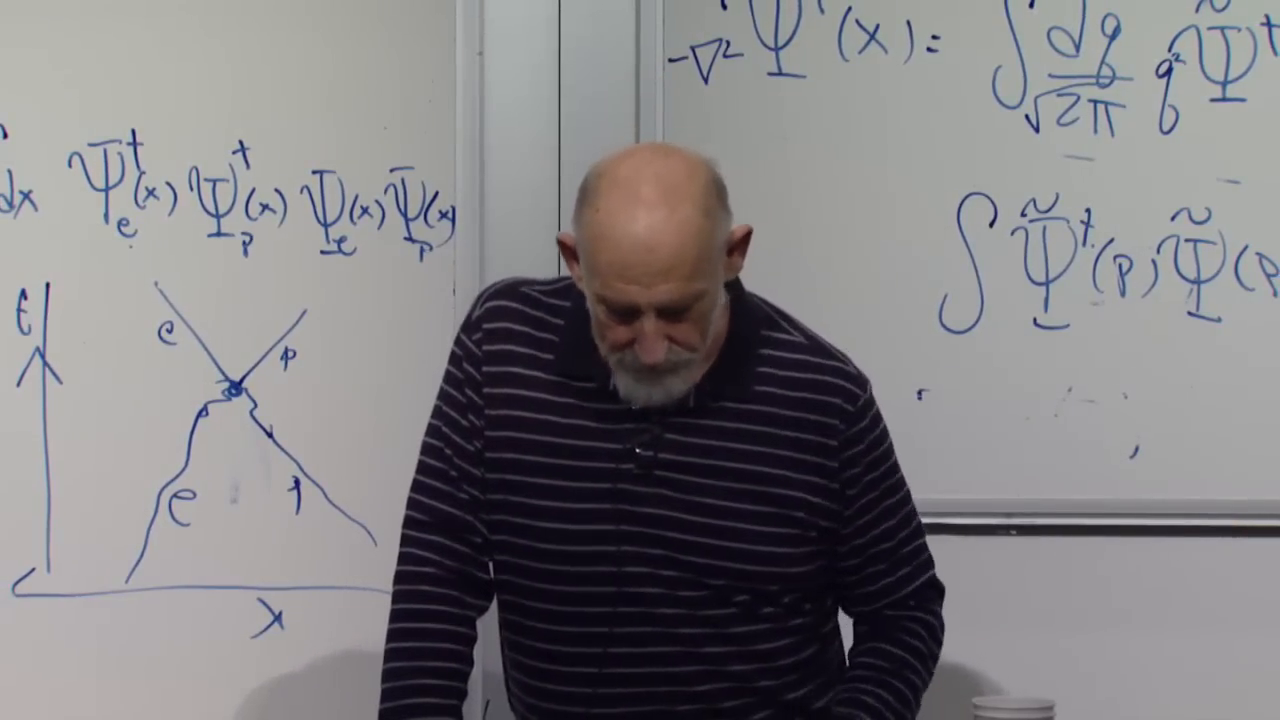
\includegraphics[width=0.94\linewidth]{lecture_09_frame_02.png}\caption{Die Kontaktwechselwirkung an der Tafel. Oberhalb der Raumzeit-Skizze stehen die vier lokalen Feldoperatoren; der Treffpunkt ist der einzige Ort, an dem die idealisierte Wechselwirkung wirkt.}\lectureframe{00:35:36}\end{figure}

\begin{figure}[htbp]\centering
\begin{tikzpicture}[x=1.2cm,y=1.0cm,>=Latex]
\draw[->] (-3.0,0) -- (3.0,0) node[right] {$x$};
\draw[->] (0,-0.2) -- (0,4.2) node[above] {$t$};
\coordinate (v) at (0,2.0);
\fill (v) circle (1.8pt);
\draw[thick,->] (-2.2,0.4) -- (v);
\draw[thick,->] (2.0,0.4) -- (v);
\draw[thick,->] (v) -- (-1.6,3.7);
\draw[thick,->] (v) -- (2.2,3.7);
\node[left] at (-1.65,0.7) {$e$};
\node[right] at (1.55,0.7) {$p$};
\node[left] at (-1.15,3.3) {$e$};
\node[right] at (1.65,3.3) {$p$};
\node[right] at (0.12,2.05) {$g$};
\end{tikzpicture}\caption{Eine klare Rekonstruktion des lokalen Streubildes. Der Vertex ist eine Kurzschreibweise für den Operator in Gl.~\eqref{eq:l9-contact}, kein klassisches Stoßgesetz.}\end{figure}

Reale Elektronen und Protonen wechselwirken über das Coulomb-Potential über eine gewisse Entfernung hinweg. Das Kontaktmodell ist lediglich ein erster, kleiner Schritt: Würde das Experiment zeigen, dass zwei Teilchensorten nur dann streuen, wenn sie sich überlappen, wäre Gl.~\eqref{eq:l9-contact} ein typischer Term, den wir in den Hamiltonoperator aufnehmen würden.

\begin{classroomqa}\lecturetimestamp{00:35:40}\audiencequestion{Warum gehört dieser Streuoperator zum Hamiltonoperator, wenn sich die Energie nicht ändert?}\lecturerresponse{Der Hamiltonoperator ist sowohl der Energieoperator als auch der Erzeuger der Zustandsänderung. Eine potentielle Energie zwischen den beiden Teilchen bewirkt Streuung während der zeitlichen Entwicklung. Die Erhaltung der Gesamtenergie bedeutet nicht, dass der Zustand oder die einzelnen Impulse der Teilchen unverändert bleiben.}\end{classroomqa}

Daraus ergibt sich eine praktische Regel. Zuerst ermitteln wir experimentell, welche lokalen Prozesse Teilchen durchlaufen können. Dann kodieren wir diese Prozesse in dem Operator, der den Zustand aktualisiert. Feldprodukte sind keine bloße algebraische Zierde: Ihre adjungierten und nicht adjungierten Faktoren legen fest, welche Teilchensorten auftreten und verschwinden.

\section{Zerfall, Umkehrprozess und Hermitizität}

Angenommen, in einer Blasenkammer endet die Spur einer Teilchensorte \(A\) an einem Punkt, von dem die Spuren \(B\) und \(C\) ausgehen. Der lokale Prozess lautet
\begin{equation}
A\longrightarrow B+C.
\end{equation}
Der Operator, der ihn bewirkt, ist
\begin{equation}
V=g\int dx\,
\psi_B^\dagger(x)\psi_C^\dagger(x)\psi_A(x).
\label{eq:l9-decay-half}
\end{equation}
Das Vernichtungsfeld entfernt \(A\); die beiden Erzeugungsfelder erzeugen \(B\) und \(C\) am selben Ort. Die Integration mit gleichem Gewicht über jedes \(x\) drückt räumliche Translationsinvarianz aus und liefert unmittelbar
\begin{equation}
p_A=p_B+p_C.
\end{equation}

Ein Hamiltonoperator muss hermitesch sein. Dadurch ist \(e^{-itH}\) unitär und die Gesamtwahrscheinlichkeit bleibt erhalten. Gleichung~\eqref{eq:l9-decay-half} ist für sich genommen nicht hermitesch, daher müssen wir ihren adjungierten Term hinzufügen:
\begin{equation}
H_{\mathrm{int}}
=\int dx\left[
g\,\psi_B^\dagger\psi_C^\dagger\psi_A
+g^*\,\psi_A^\dagger\psi_C\psi_B
\right](x).
\label{eq:l9-hermitian-vertex}
\end{equation}
Für eine reelle Kopplung \(g\) sind die beiden Koeffizienten gleich. Beim hermiteschen Konjugieren wird neben dem Austausch von adjungierten und nicht adjungierten Feldern auch die Operatorreihenfolge umgekehrt. In diesem bosonischen Spielzeugmodell kommutieren Felder verschiedener Teilchensorten, sodass diese Umordnung keine weitere Schwierigkeit mit sich bringt.

Der zweite Term beschreibt den umgekehrten Prozess,
\begin{equation}
B+C\longrightarrow A.
\end{equation}
Ein geschlossener, unitärer Hamiltonoperator, der den Zerfall zulässt, enthält also auch die Amplitude für die Rekombination. Das bedeutet nicht, dass beide Richtungen bei jeder Wahl der äußeren Impulse auftreten; Energieerhaltung und andere Erhaltungssätze können eine Richtung kinematisch unmöglich machen. Es bedeutet, dass sowohl der Operator als auch sein Adjungierter zur Dynamik gehören.

\begin{classroomqa}\lecturetimestamp{00:42:48}\audiencequestion{Kann es eine Ausnahme von der Regel geben, dass auch der umgekehrte Prozess möglich ist?}\lecturerresponse{Nicht bei einem hermiteschen Hamiltonoperator eines geschlossenen Systems: Die adjungierte Wechselwirkung ist erforderlich. Eine bestimmte Rückreaktion kann durch die Kinematik oder eine andere erhaltene Quantenzahl dennoch blockiert sein, aber das konjugierte Matrixelement ist vorhanden.}\end{classroomqa}

Die Zahl \(g\) ist die Kopplungskonstante. Ist \(g\) klein, wechselwirken Teilchen, die aufeinandertreffen, nur schwach; ist sie groß, ist die Übergangsamplitude größer. Kopplungskonstanten sind in der Regel experimentell bestimmte Parameter, obwohl Symmetrien mehrere scheinbar verschiedene Kopplungen miteinander verknüpfen können.

Dieselbe Grammatik lässt sich auf kompliziertere Reaktionen anwenden. Beim Betazerfall
\begin{equation}
n\longrightarrow p+e^-+\bar\nu_e,
\end{equation}
enthält ein schematischer lokaler Term vier Felder: Eines vernichtet das Neutron, drei erzeugen Proton, Elektron und Elektron-Antineutrino; hinzu kommt der hermitesch konjugierte Prozess. Schon daran ist zu erkennen, wie eine kleine Menge von Operator-Monomeren allmählich eine Quantenfeldtheorie definiert.

\section{Warum das Quadrat des Hamiltonoperators wichtig ist}

Die Kurzzeitformel \eqref{eq:l9-short-update} berücksichtigte nur die erste Ordnung in \(\epsilon\). Die vollständige Entwicklung lautet
\begin{equation}
e^{-i\epsilon H}
=1-i\epsilon H-\frac{\epsilon^2}{2}H^2
+\frac{i\epsilon^3}{3!}H^3+\cdots.
\label{eq:l9-exponential}
\end{equation}
In zweiter Ordnung wirkt der Hamiltonoperator zweimal. Das ist der algebraische Ursprung der ersten zusammengesetzten Prozessbilder.

Beim Vertex \(A\leftrightarrow B+C\) kann eine Wirkung \(B+C\) zu \(A\) verbinden und eine zweite dieses \(A\) wieder in \(B+C\) zerlegen:
\begin{equation}
B+C\longrightarrow A\longrightarrow B+C.
\label{eq:l9-bc-scattering}
\end{equation}
Der Gesamtbeitrag ist eine Streuamplitude \(B+C\to B+C\). Das Zwischenzustands-\(A\) ist kein zusätzliches beobachtetes Ereignis; es bezeichnet den Zustand, über den zwischen den beiden Wirkungen der Wechselwirkung summiert wird.

\begin{classroomqa}\lecturetimestamp{00:49:54}\audiencequestion{Muss das \(C\)-Feld im hingeschriebenen Produkt zweiter Ordnung adjungiert sein?}\lecturerresponse{Ja, die Operatorreihenfolge muss der angegebenen Abfolge entsprechen. Der erste Vertex vernichtet \(B\) und \(C\) und erzeugt \(A\); der zweite vernichtet \(A\) und erzeugt erneut \(B\) und \(C\). Mit den entsprechenden Adjungierten ist diese Deutung wiederhergestellt.}\end{classroomqa}

\begin{figure}[htbp]\centering
\includegraphics[width=0.94\linewidth]{lecture_09_frame_05.png}\caption{Die beiden Orientierungen des elementaren \(A\leftrightarrow B+C\)-Vertex an der Tafel. Ihre Kombination ist die bildliche Kurzschreibweise für den Prozess zweiter Ordnung in Gl.~\eqref{eq:l9-bc-scattering}.}\lectureframe{00:48:56}\end{figure}

Nun kommt ein Zuschauer-\(B\) hinzu. Eine Wirkung lässt \(A\) \(C\) emittieren und zu \(B\) werden; eine spätere Wirkung lässt dieses \(C\) sich mit dem ursprünglichen \(B\) verbinden, sodass \(A\) entsteht. Die äußeren Teilchen sind wieder \(A+B\), doch ihre Impulse können sich ändern. Wir beschreiben dies als Streuung von \(A\) und \(B\) durch den Austausch von \(C\).

\begin{figure}[htbp]\centering
\includegraphics[width=0.94\linewidth]{lecture_09_frame_06.png}\caption{Die Austausch-Konstruktion an der Tafel. Im Diagramm rechts verbinden eine interne \(C\)-Linie und zwei elementare Vertices die Streuung der äußeren \(A\)- und \(B\)-Teilchen.}\lectureframe{00:51:22}\end{figure}

\begin{figure}[htbp]\centering
\begin{tikzpicture}[x=1.1cm,y=1cm,>=Latex]
\draw[->] (-3.7,-0.2) -- (-3.7,4.2) node[above] {$t$};
\coordinate (v1) at (-0.9,1.25);
\coordinate (v2) at (0.9,2.95);
\fill (v1) circle (1.7pt);
\fill (v2) circle (1.7pt);
\draw[thick,->] (-2.6,0.2) -- (v1) node[midway,below left] {$A$};
\draw[thick,->] (2.6,0.2) -- (v2) node[midway,below right] {$B$};
\draw[thick,->] (v1) -- (-2.4,4.0) node[midway,left] {$B$};
\draw[thick,->] (v2) -- (2.5,4.0) node[midway,right] {$A$};
\draw[thick,->,dashed] (v1) -- (v2) node[midway,above left] {$C$};
\node[below] at (0,-0.05) {$A+B\rightarrow A+B$};
\end{tikzpicture}\caption{Eine klare Rekonstruktion des \(C\)-Austauschs. Jeder Punkt liefert einen Faktor \(g\), daher ist dieser Beitrag zweiter Ordnung proportional zu \(g^2\).}\end{figure}

Jeder lokale Wechselwirkungspunkt heißt Vertex. Jeder Vertex trägt einen Faktor seiner Kopplung bei. Ein Beitrag mit zwei Vertices enthält also \(g^2\), einer mit drei Vertices \(g^3\) und so weiter. Ein einziger Term im Hamiltonoperator korreliert somit eine große Familie von Reaktionen. Diese Ökonomie ist ein Grund für die große Leistungsfähigkeit der Quantenfeldtheorie: Eine kleine Zahl lokaler Wechselwirkungen ordnet eine enorme Menge von Streudaten.

\begin{classroomqa}\lecturetimestamp{00:53:14}\audiencequestion{Wie nennt man den Prozess \(A\to B+C\to A\)?}\lecturerresponse{Es handelt sich um einen Selbstenergiebeitrag. Ein beobachtetes \(A\) ist nicht einfach der ungestörte Einteilchen-Basiszustand; der Wechselwirkungszustand enthält auch Amplituden für nahegelegene \(B+C\)-Komponenten. Streuung daran kann diese bekleidete Struktur sichtbar machen.}\end{classroomqa}

Die Quantenelektrodynamik liefert das vertraute Beispiel. Ein lokaler Elektron--Photon-Vertex kann ein Elektron vernichten, ein Elektron neu erzeugen und ein Photon erzeugen. In zweiter Ordnung kann das Elektron ein Photon emittieren und wieder absorbieren. Es liegt nahe, dies als winzigen Film zu erzählen, doch seine präzise Bedeutung ist ein Term in der Störungsentwicklung. Das physikalische Elektron ist ein bekleideter Zustand mit Komponenten, die Photonen enthalten.

Die Abschätzung aus der Vorlesung, diese Komponente betrage ``etwa ein Prozent'', vermittelt die Größenordnung, die durch die Feinstrukturkonstante \(\alpha_{\mathrm{em}}\simeq 1/137\) festgelegt wird. Eine präzise Wahrscheinlichkeit für eine Photon-Fock-Komponente hängt von der Energieauflösung und davon ab, wie der Wechselwirkungszustand definiert wird; sie ist keine universelle Ein-Prozent-Eigenschaft eines isolierten Elektrons. Die belastbare Aussage ist, dass die Wechselwirkung die messbare Struktur des Elektrons verändert.

\section{Was ein Diagramm aussagt und was nicht}

Die Diagramme sind eine rechnerische Kurzschreibweise für Potenzen des Wechselwirkungs-Hamiltonoperators. Sie sind keine verlässlichen klassischen Abläufe, in denen ein Teilchen eindeutig erst ein Ereignis und dann ein anderes durchläuft. Wenn man hineinschaut, um zu entscheiden, was ``wirklich geschehen'' ist, verändert man das Experiment und zerstört die kohärente Summe, wie bei gewöhnlicher Quanteninterferenz.

\begin{classroomqa}\lecturetimestamp{00:56:52}\audiencequestion{Sind an jedem Vertex sowohl Energie als auch Impuls erhalten?}\lecturerresponse{Bei der hier durchgeführten Hamilton-Konstruktion zu gleichen Zeiten ergibt das räumliche Integral unmittelbar eine Impuls-Deltafunktion. Für diese einzelne Einfügung hat noch kein Zeitintegral eine Energie-Deltafunktion geliefert. Die vollständige, translationsinvariante Streuamplitude erhält die Gesamtenergie, während interne Linien nicht der On-Shell-Beziehung beobachteter Teilchen entsprechen müssen. In der kovarianten Diagrammsprache ist der Viererimpuls an jedem Vertex erhalten, interne Teilchen können jedoch off shell sein.}\end{classroomqa}

Die scheinbar fehlende Energie in einem naiven Vertexbild ist ein weiterer Grund, die Wechselwirkungsenergie nicht zu vernachlässigen. Der gesamte Hamiltonoperator ist mehr als die Summe der Energien freier Teilchen. Falls Verwirrung entsteht, kehren wir zu Gl.~\eqref{eq:l9-exponential} zurück: Das Bild steht für einen Term in der Entwicklung der unitären zeitlichen Entwicklung. Die vollständige Feynman-Diagrammtechnik liefert systematische Zeitordnung, Propagatoren, Integrationen und Symmetriefaktoren, doch die grundlegende Physik beginnt bereits hier.

Eine weiterführende Frage nimmt das Diagramm zu wörtlich und vergleicht das emittierte Photon mit dem elektrischen Feld, das ein langsam bewegtes Elektron umgibt.

\begin{classroomqa}\lecturetimestamp{00:58:26}\audiencequestion{Wird das elektrische Feld des Elektrons in einiger Entfernung tatsächlich von ausgestrahlten Photonen erzeugt? Wie passt das zu Interferenz und zum Aharon---Bohm-Effekt?}\lecturerresponse{Ein statisches Feld oder ein Induktionsfeld ist kein Strom realer ausgestrahlter Photonen. Die Quantenelektrodynamik beschreibt sowohl Strahlung als auch die elektromagnetische Bekleidung des Elektrons mit demselben Feld, doch die zugehörigen Quantenzustände und die Kinematik unterscheiden sich. Bei einem ultrarelativistischen Elektron lassen sich manche Feldkomponenten sinnvoll als Strom nahezu reeller Photonen auffassen; bei einem langsamen Elektron ist eine wörtliche Photonentrajektorie das falsche Modell. Der Doppelspaltversuch und der Aharon---Bohm-Effekt sind ebenfalls nichtklassische Feldphänomene, machen dieses Selbstenergie-Diagramm aber nicht zu einem mechanischen Film.}\end{classroomqa}

\begin{classroomqa}\lecturetimestamp{01:01:28}\audiencequestion{Warum scheitert ein klassisches Modell des Diagramms genau?}\lecturerresponse{Weil die Rechnung die Amplituden aller zulässigen Zwischenalternativen kohärent addiert. Die Erfahrung macht die Bilder anschaulich, doch ihr wörtlicher Gehalt geht nie über die Operatorentwicklung hinaus, durch die sie definiert sind. Sie sind eine kompakte Methode, \(H^2,H^3,\ldots\) zu berechnen, keine Aufzeichnung beobachteter Zwischenereignisse.}\end{classroomqa}

\begin{classroomqa}\lecturetimestamp{01:03:04}\audiencequestion{Kann die gewöhnliche Coulomb-Wechselwirkung als klassischer Grenzfall des Photonenaustauschs entstehen?}\lecturerresponse{Ja. Wertet man die entsprechende photonvermittelte Amplitude aus und nimmt den nichtrelativistischen statischen Grenzfall, erhält man das Coulomb-Potential. Die Herleitung ist technischer als die vorliegende Operator-Skizze und sollte dennoch nicht so verstanden werden, als spränge ein Photon buchstäblich zwischen zwei klassischen Teilchen hin und her.}\end{classroomqa}

\begin{classroomqa}\lecturetimestamp{01:03:44}\audiencequestion{Werden Kopplungskonstanten aus den Feldprodukten berechnet?}\lecturerresponse{Ihre Zahlenwerte sind gewöhnlich experimentelle Eingangsgrößen. Symmetrien können sie einschränken oder Kopplungen miteinander verknüpfen, die andernfalls unabhängig wären. Wenn eine solche Beziehung die relativen Stärken verschiedener Reaktionen vorhersagt und das Experiment sie bestätigt, ist diese Übereinstimmung besonders aufschlussreich.}\end{classroomqa}

\begin{classroomqa}\lecturetimestamp{01:04:48}\audiencequestion{Welche Rolle spielt eine zufällige Symmetrie im Vergleich zu einer Eichsymmetrie?}\lecturerresponse{Eine Eichsymmetrie schränkt unmittelbar die zulässige Struktur und die Beziehungen zwischen Kopplungen ein. Eine zufällige Symmetrie wird nicht auf fundamentaler Ebene auferlegt, sondern entsteht, weil zufällig alle zulässigen Wechselwirkungen niedriger Ordnung sie respektieren. Sie kann dennoch wichtige Folgen haben, auch wenn ihr Ursprung und ihre Robustheit sich von denen einer Eichsymmetrie unterscheiden.}\end{classroomqa}

Damit lassen wir die nichtrelativistische Feldtheorie vorerst hinter uns. Wir haben Fermionen angekündigt. Statt sie sofort zweitzuquantisieren, wollen wir zunächst die relativistische Einteilchengleichung verstehen, der ihre Feldoperatoren genügen müssen.

\section{Warum das Elektron eine relativistische Beschreibung erfordert}

Wir beginnen mit einer räumlichen Dimension. Das ist keine realistische Einschränkung, beseitigt aber die geometrische Komplexität des dreidimensionalen Spins, während die wesentliche Algebra erhalten bleibt. Das Elektron ist leicht genug, dass relativistische Effekte bereits in Atomen eine Rolle spielen. In Wasserstoff beträgt seine charakteristische Geschwindigkeit etwa
\begin{equation}
v\sim\alpha_{\mathrm{em}}c\approx 0.007c,
\end{equation}
also ungefähr ein Prozent der Lichtgeschwindigkeit. Bei inneren Elektronen eines schweren Atoms liegt die grobe Größenordnung bei \(v\sim Z\alpha_{\mathrm{em}}c\), sodass relativistische Korrekturen erheblich sein können. Ob historische Neugier oder die für die Atomphysik erforderliche Genauigkeit den entscheidenden Anstoß gab: Eine relativistische Gleichung vom Schr\"odinger-Typ ist physikalisch notwendig.

Das übliche Quantisierungsrezept geht von der klassischen Beziehung zwischen Energie und Impuls aus. Nichtrelativistisch gilt
\begin{equation}
E=\frac{p^2}{2m},
\end{equation}
und die Ersetzungen
\begin{equation}
E\mapsto i\partial_t,
\qquad
p\mapsto-i\partial_x
\end{equation}
ergeben
\begin{equation}
i\partial_t\varphi(x,t)
=-\frac{1}{2m}\partial_x^2\varphi(x,t).
\end{equation}

Die Relativitätstheorie liefert dagegen mit \(c=1\)
\begin{equation}
E^2=p^2+m^2.
\label{eq:l9-rel-dispersion}
\end{equation}

\begin{figure}[htbp]\centering
\includegraphics[width=0.94\linewidth]{lecture_09_frame_07.png}\caption{Der Übergang an der Tafel von \(E=p^2/2m\) zur relativistischen Beziehung \(E^2=p^2+m^2\), mit \(c=1\).}\lectureframe{01:10:30}\end{figure}

Wenden wir die Ersetzungen auf die quadrierte Beziehung an, erhalten wir
\begin{equation}
-\partial_t^2\varphi
=\left(-\partial_x^2+m^2\right)\varphi,
\label{eq:l9-klein-gordon}
\end{equation}
oder äquivalent
\begin{equation}
\left(\partial_t^2-\partial_x^2+m^2\right)\varphi=0.
\end{equation}
Dies ist die Klein---Gordon-Gleichung. Sie ist eine durchaus sinnvolle relativistische Feldgleichung, insbesondere für Felder mit Spin null. Die gesuchte Elektronengleichung soll jedoch erster Ordnung in der Zeit sein,
\begin{equation}
i\partial_t\Psi=H\Psi,
\end{equation}
sodass \(H\) selbst die zeitliche Entwicklung erzeugt und nicht nur \(H^2\).

Formal könnte man
\begin{equation}
H=\sqrt{-\partial_x^2+m^2}.
\end{equation}
wählen. Die Wurzel lässt sich im Impulsraum eindeutig definieren, wo sie mit \(\sqrt{p^2+m^2}\) multipliziert, doch im Ortsraum ist sie ein nichtlokaler pseudodifferentieller Operator. Mathematisch ist das sinnvoll, für die lokale Gleichung, die wir suchen, aber ästhetisch unbefriedigend. Deshalb beginnen wir noch einmal von vorn.

\section{Eine masselose Welle, die sich nach rechts bewegt}

Betrachten wir zunächst ein masseloses Teilchen, das sich nach rechts bewegt. Für seine positive Energie und seinen Impuls gilt
\begin{equation}
E=p
\qquad (c=1).
\end{equation}
Die Quantisierung ergibt
\begin{equation}
i\partial_t\psi=-i\partial_x\psi,
\end{equation}
oder
\begin{equation}
(\partial_t+\partial_x)\psi=0.
\label{eq:l9-right-mover}
\end{equation}
Jede Lösung hat die Form
\begin{equation}
\psi(x,t)=f(x-t).
\end{equation}
Das Profil bleibt unverändert und bewegt sich mit Lichtgeschwindigkeit nach rechts.

Dabei treten sofort zwei Schwierigkeiten auf. Erstens hat ein negativer Impuls, wenn Gl.~\eqref{eq:l9-right-mover} auf beliebige Fourier-Moden wirken darf, die Energie \(E=p<0\); der Hamiltonoperator ist dann nach unten nicht beschränkt. Eine willkürliche Beschränkung auf \(p>0\) würde nur rechtslaufende Moden beibehalten und ergäbe noch nicht die gesuchte Elektronentheorie. Zweitens ist die Gleichung eine Einbahnstraße: Sie enthält kein gewöhnliches linkslaufendes Elektron. Zunächst lösen wir das Links-rechts-Problem und lassen die negativen Energien außer Betracht.

\section{Zwei Komponenten und die Alpha-Matrix}

Wir führen zwei Amplituden ein,
\begin{equation}
\Psi(x,t)=
\begin{pmatrix}
\psi_1(x,t)\\[3pt]
\psi_2(x,t)
\end{pmatrix},
\end{equation}
wobei \(\psi_1\) im masselosen Grenzfall nach rechts und \(\psi_2\) nach links läuft:
\begin{align}
(\partial_t+\partial_x)\psi_1&=0,
&
(\partial_t-\partial_x)\psi_2&=0.
\end{align}
Die Quantenmechanik erlaubt zudem beliebige Überlagerungen der beiden. Ein Teilchen kann daher Amplituden für beide Richtungen haben, statt ein für alle Mal ein klassisches Etikett zu tragen.

Dieser zusätzliche zweifachwertige Freiheitsgrad ähnelt algebraisch dem Spin, ist aber in einer Dimension kein gewöhnlicher Drehimpuls. Definieren wir
\begin{equation}
\alpha=
\begin{pmatrix}
1&0\\
0&-1
\end{pmatrix}
=\sigma_3.
\label{eq:l9-alpha}
\end{equation}
Der Eigenvektor zum Eigenwert \(+1\) wählt die rechts laufende Komponente aus, der zum Eigenwert \(-1\) die links laufende. In der masselosen Theorie lautet der Hamiltonoperator einfach
\begin{equation}
H=\alpha p,
\end{equation}
und die beiden Gleichungen lassen sich zu einer einzigen zusammenfassen:
\begin{equation}
i\partial_t\Psi=-i\alpha\partial_x\Psi.
\label{eq:l9-massless-dirac}
\end{equation}

\begin{classroomqa}
\lecturetimestamp{01:22:44}
\audiencequestion{Wie heißt die Diagonalmatrix, die die beiden Komponenten unterscheidet?}
\lecturerresponse{Als Pauli-Matrix ist sie \(\sigma_3\), nicht \(\sigma_1\). In der Dirac-Notation für die vorliegende Konstruktion nennen wir sie \(\alpha\). Ihre Algebra ist die bekannte Pauli-Algebra, obwohl sie hier die Richtung und nicht den Drehimpuls bezeichnet.}
\end{classroomqa}

\begin{classroomqa}
\lecturetimestamp{01:23:32}
\audiencequestion{Erhält die Konstruktion in drei Dimensionen, wo die Richtung ein Vektor ist, eine stärker geometrische Bedeutung?}
\lecturerresponse{Ja. Das dreidimensionale Problem erfordert eine Matrix für jede Raumrichtung und führt zu einer reichhaltigeren Spinorstruktur. Das eindimensionale Modell ist in seinem eigenen Rahmen dennoch exakt und isoliert die wesentliche Links-rechts-Algebra, ohne diese zusätzliche Komplexität.}
\end{classroomqa}

\begin{figure}[htbp]
\centering
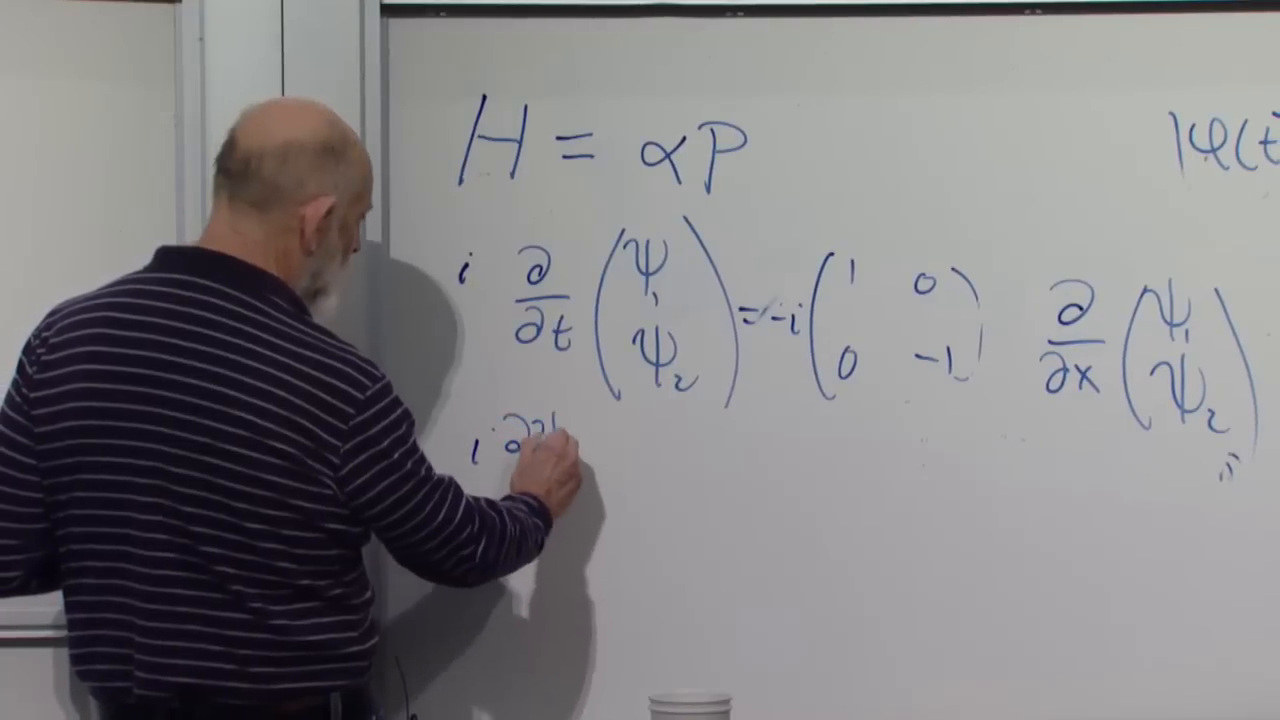
\includegraphics[width=0.94\linewidth]{lecture_09_frame_03.png}
\caption{Die masselose Zweikomponentengleichung an der Tafel: \(H=\alpha P\); die Diagonalmatrix ordnet \(\psi_1\) und \(\psi_2\) entgegengesetzte Ausbreitungsrichtungen zu.}
\lectureframe{01:26:00}
\end{figure}

Das Problem der Bewegung nur in eine Richtung ist behoben. Das Spektrum negativer Energien bleibt bestehen, und wir haben einen dritten Mangel entdeckt: Die beiden Komponenten sind weiterhin masselos und breiten sich mit Lichtgeschwindigkeit aus. Im nächsten Schritt müssen eine Ruheenergie eingeführt und die Richtungen gekoppelt werden.

\section{Masse hinzufügen und die Dirac-Algebra entdecken}

Fügen wir den allgemeinsten einfachen, zur Masse proportionalen Term hinzu:
\begin{equation}
H=\alpha p+\beta m,
\label{eq:l9-dirac-hamiltonian}
\end{equation}
wobei \(\beta\) nur auf den zweikomponentigen Index wirkt. Es hätte die Einheitsmatrix oder eine andere Matrix sein können; wir lassen die relativistische Dispersionsrelation entscheiden.

Da \(H^2\) gleich \(p^2+m^2\) sein muss, quadrieren wir Gl.~\eqref{eq:l9-dirac-hamiltonian}:
\begin{align}
H^2
&=(\alpha p+\beta m)^2\\
&=\alpha^2p^2+\beta^2m^2
+(\alpha\beta+\beta\alpha)pm.
\label{eq:l9-square-dirac}
\end{align}
Die Matrizen kommutieren mit \(p\), weil sie auf den internen zweikomponentigen Raum wirken, während \(p\) auf die räumliche Wellenfunktion wirkt. Damit Gl.~\eqref{eq:l9-rel-dispersion} erfüllt ist, muss gelten:
\begin{equation}
\alpha^2=\mathbb{1},
\qquad
\beta^2=\mathbb{1},
\qquad
\{\alpha,\beta\}
=\alpha\beta+\beta\alpha=0.
\label{eq:l9-dirac-algebra}
\end{equation}
Die erste Bedingung ist für \(\alpha=\sigma_3\) bereits erfüllt. Jede andere Pauli-Matrix antikommutiert mit ihr und hat das Quadrat der Einheitsmatrix. Wir wählen
\begin{equation}
\beta=
\begin{pmatrix}
0&1\\
1&0
\end{pmatrix}
=\sigma_1.
\label{eq:l9-beta}
\end{equation}
Die Wahl von \(\sigma_1\) statt \(\sigma_2\) ist eine Konvention für die Basis; nach einer unitären Basisänderung realisieren beide dieselbe Algebra.

\begin{classroomqa}
\lecturetimestamp{01:33:00}
\audiencequestion{Hat Dirac einfach erkannt, dass Pauli-Matrizen diese algebraischen Bedingungen erfüllen?}
\lecturerresponse{Die historische Herleitung wurde direkt in drei Dimensionen durchgeführt und führte Matrizen ein, die die erforderlichen Relationen erfüllen. Sobald die Bedingungen formuliert sind, ergibt sich die eindimensionale Lösung unmittelbar aus der Pauli-Algebra: Man wählt zwei verschiedene Pauli-Matrizen.}
\end{classroomqa}

\begin{classroomqa}
\lecturetimestamp{01:34:24}
\audiencequestion{Ist dieses \(\beta\) der relativistische Geschwindigkeitsparameter \(v/c\)?}
\lecturerresponse{Nein. Es ist eine Matrix, die auf die Spinorkomponenten wirkt. Der wiederverwendete Buchstabe ist lediglich Diracs Notation; mit der kinematischen Größe \(v/c\) hat er nichts zu tun.}
\end{classroomqa}

In drei Raumdimensionen reichen \(2\times2\)-Matrizen für den vollständigen Satz der erforderlichen antikommutierenden Matrizen nicht aus. Diese Erweiterung wird auf später verschoben. In einer Dimension genügen die Gleichungen ~\eqref{eq:l9-alpha} und \eqref{eq:l9-beta}.

\section{Die gekoppelte eindimensionale Dirac-Gleichung}

Setzen wir \(p=-i\partial_x\) ein, erhalten wir die eindimensionale Dirac-Gleichung in Hamilton-Form:
\begin{equation}
i\partial_t\Psi
=\left(-i\alpha\partial_x+\beta m\right)\Psi.
\label{eq:l9-one-dimensional-dirac}
\end{equation}
Da \(\alpha\) diagonal ist, lässt ihr Ableitungsterm die beiden Komponenten getrennt. Da \(\beta\) nicht diagonal ist, vertauscht der Massenterm sie. In Komponenten geschrieben:
\begin{align}
i\partial_t\psi_1
&=-i\partial_x\psi_1+m\psi_2,
\label{eq:l9-dirac-component-one}\\
i\partial_t\psi_2
&=+i\partial_x\psi_2+m\psi_1.
\label{eq:l9-dirac-component-two}
\end{align}

\begin{figure}[htbp]
\centering
\includegraphics[width=0.94\linewidth]{lecture_09_frame_08.png}
\caption{Die gekoppelten Komponentengleichungen an der Tafel. Die entgegengesetzten Vorzeichen der Ableitungen kodieren die Rechts- und Linksbewegung; der nichtdiagonale Massenterm vertauscht \(\psi_1\) und \(\psi_2\).}
\lectureframe{01:37:44}
\end{figure}

Sobald \(m\ne0\), entwickeln sich die Komponenten nicht mehr unabhängig voneinander. Durch Quadrieren der Gleichung erster Ordnung erhält man für jede Komponente den Klein--Gordon-Operator:
\begin{equation}
\left(\partial_t^2-\partial_x^2+m^2\right)\psi_a=0,
\qquad a=1,2,
\end{equation}
Für ebene Wellen gilt \(E^2=p^2+m^2\). Ihre Gruppengeschwindigkeit ist
\begin{equation}
v_g=\frac{dE}{dp}=\frac{p}{E},
\end{equation}
und ihr Betrag ist bei von null verschiedener Masse kleiner als eins.

Der Zusammenhang zwischen Masse und Mischung der Links- und Rechtskomponenten ist kein Zufall. Ein masseloser Rechtshänder bleibt unter jeder eigentlichen Lorentz-Boost-Transformation ein Rechtshänder; kein Beobachter mit unterlichtschneller Geschwindigkeit kann das Licht überholen und seine Richtung umkehren. Ein massives Teilchen lässt sich in sein Ruhesystem überführen. Betrachtet man es dann aus einem schnelleren Bezugssystem, das sich in derselben Richtung bewegt, erscheint seine Geschwindigkeit umgekehrt. Eine relativistische Theorie mit Masse kann die rechts und links laufenden Sektoren daher nicht dauerhaft getrennt halten. Der nichtdiagonale Massenterm liefert genau die erforderliche Kopplung.

\begin{classroomqa}
\lecturetimestamp{01:40:01}
\audiencequestion{Ist der Austausch der beiden Komponenten eine chirale Oszillation?}
\lecturerresponse{In dieser eindimensionalen Basis unterscheidet \(\alpha\) die beiden masselosen chiralen Richtungen. Der Massenterm ist nichtdiagonal und mischt sie, sodass die Chiralität nicht mehr erhalten ist. In diesem Sinne ist der Massenterm die Ursache der chiralen Oszillation.}
\end{classroomqa}

\begin{classroomqa}
\lecturetimestamp{01:40:46}
\audiencequestion{Warum sollte eine Fermionengleichung die Quadratwurzel einer Bosonengleichung sein?}
\lecturerresponse{Das sollte man nicht so verstehen. Die Dispersionsrelation \(E^2=p^2+m^2\) gilt für jedes freie relativistische Teilchen, unabhängig von seiner Statistik. Der Dirac-Operator liefert zufällig eine Matrixfaktorisierung des Klein--Gordon-Operators, aber aus dieser algebraischen Beziehung werden keine Fermionen aus Bosonen hergeleitet.}
\end{classroomqa}

\begin{classroomqa}
\lecturetimestamp{01:41:31}
\audiencequestion{Lässt sich die Gleichung in eine einfache skalare Faktorisierung in getrennte links und rechts laufende Faktoren zerlegen?}
\lecturerresponse{Nur im masselosen Grenzfall entkoppeln sich die beiden chiralen Gleichungen zu unabhängigen skalaren Faktoren. Für \(m\ne0\) ist die nützliche Faktorisierung matrixwertig: Die antikommutierenden Matrizen \(\alpha\) und \(\beta\) beseitigen den unerwünschten Mischterm.}
\end{classroomqa}

\begin{classroomqa}
\lecturetimestamp{01:42:04}
\audiencequestion{Bilden diese beiden gekoppelten Gleichungen bereits die Dirac-Gleichung?}
\lecturerresponse{Ja. Zusammen bilden sie die Dirac-Gleichung in einer Raumdimension, äquivalent zur kompakten Form in Gl.~\eqref{eq:l9-one-dimensional-dirac}. Eine symmetrischere kovariante Notation erhält man durch Multiplikation mit \(\beta\); diese Form behandeln wir jedoch später.}
\end{classroomqa}

Zwei Aufgaben bleiben bewusst ungelöst. Die Konstruktion hat die negativen Energien nicht beseitigt; sie hat negative Energielösungen in beiden Richtungssektoren geliefert, sodass dieses Problem nun deutlicher hervortritt. Außerdem lebt die Theorie weiterhin in einer Raumdimension. Die Interpretation der negativen Energielösungen und die Erweiterung der Matrixalgebra auf \(3+1\) Dimensionen sind die nächsten Schritte.
